% !TEX program = xelatex
% Figure 1 (CONSORT 형식, nested CV, 단순화 판): 환자 선정과 outer·inner 분할 인원.
% 주 흐름은 세로 한 줄, outer test 는 오른쪽 가지. 수치 출처는 fig1_patient_flowchart_nested.tex 머리말에 있다.
\documentclass[tikz,border=8pt,10pt]{standalone}
\usepackage{fontspec}
\IfFontExistsTF{Times New Roman}{\setmainfont{Times New Roman}}{\setmainfont{Nimbus Roman}}
\usetikzlibrary{arrows.meta,positioning}
\begin{document}
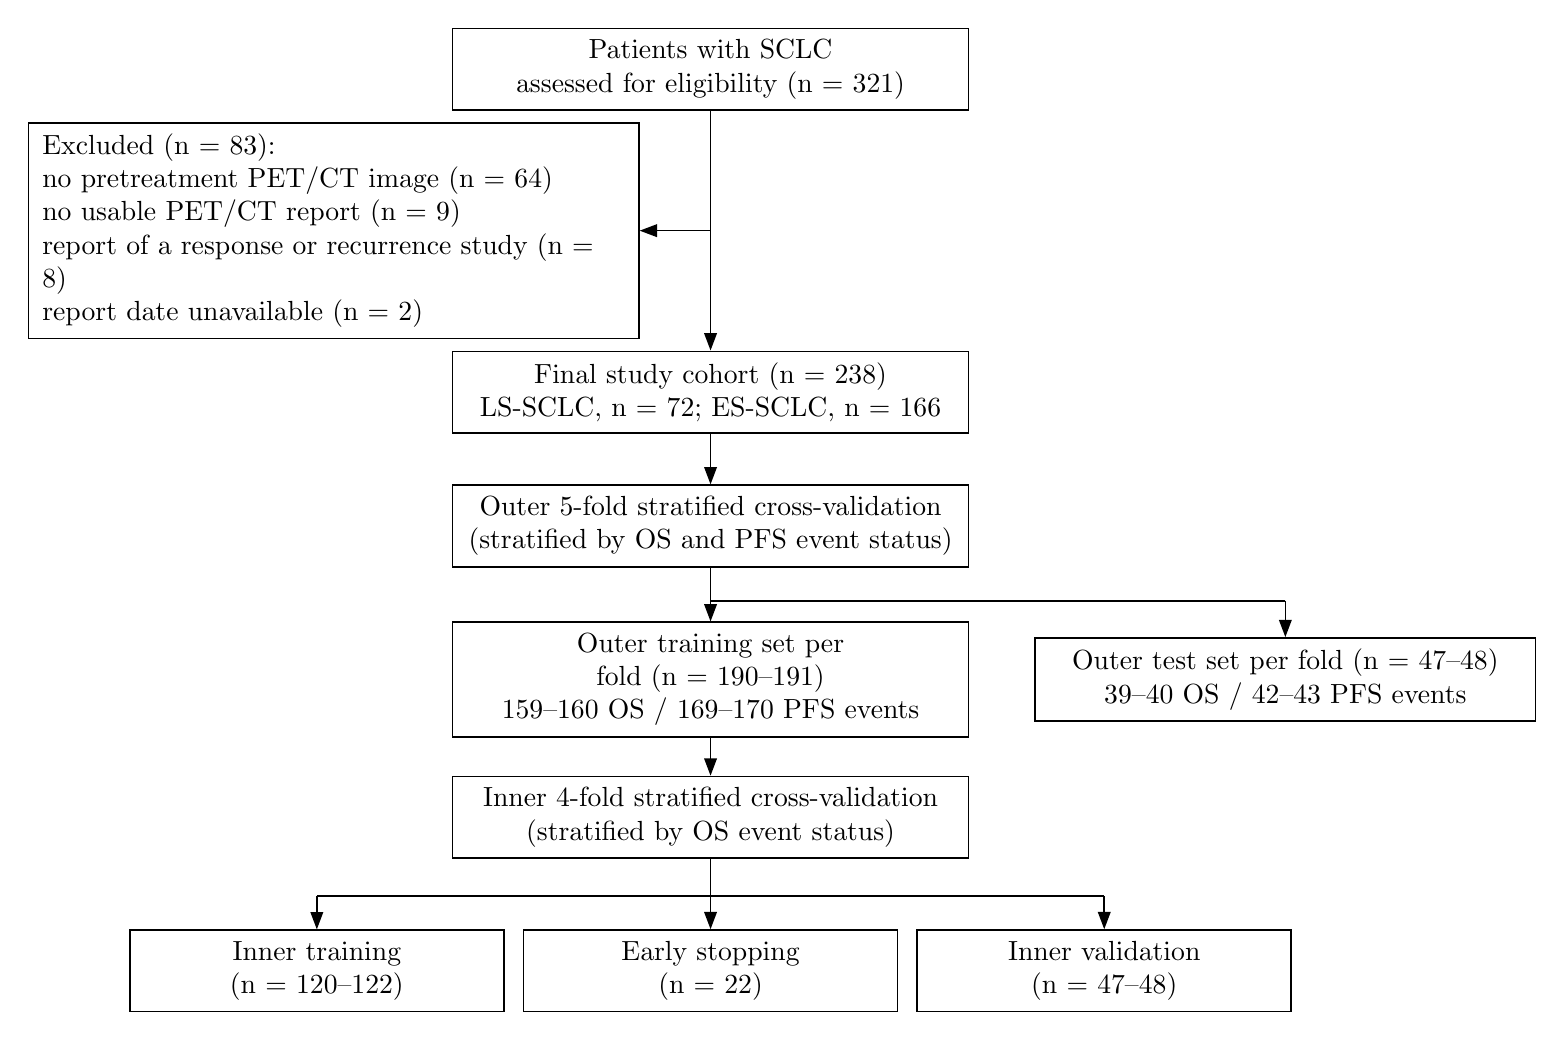
\begin{tikzpicture}[x=1cm,y=1cm,
  box/.style={draw=black, line width=0.6pt, fill=white, align=center,
              inner xsep=5pt, inner ysep=4pt, text width=#1},
  box/.default=62mm,
  excl/.style={box=74mm, align=left},
  sub/.style={box=44mm},
  arr/.style={draw=black, line width=0.6pt, -{Triangle[length=2.2mm,width=1.6mm]}},
  line/.style={draw=black, line width=0.6pt},
]

% ---------------- 선정 ----------------
\node[box] (all) at (0,0)
  {Patients with SCLC\\ assessed for eligibility (n = 321)};

\node[excl, anchor=east] (ex) at (-0.9,-2.05)
  {Excluded (n = 83):\\
   no pretreatment PET/CT image (n = 64)\\
   no usable PET/CT report (n = 9)\\
   report of a response or recurrence study (n = 8)\\
   report date unavailable (n = 2)};

\node[box] (final) at (0,-4.1)
  {Final study cohort (n = 238)\\ LS-SCLC, n = 72; ES-SCLC, n = 166};

% ---------------- nested 교차검증 ----------------
\node[box] (cv) at (0,-5.8)
  {Outer 5-fold stratified cross-validation\\ (stratified by OS and PFS event status)};

\node[box] (otr) at (0,-7.75)
  {Outer training set per fold (n = 190--191)\\ 159--160 OS / 169--170 PFS events};
\node[box=60mm] (ote) at (7.3,-7.75)
  {Outer test set per fold (n = 47--48)\\ 39--40 OS / 42--43 PFS events};

\node[box] (icv) at (0,-9.5)
  {Inner 4-fold stratified cross-validation\\ (stratified by OS event status)};

\node[sub] (itr) at (-5.0,-11.45) {Inner training\\ (n = 120--122)};
\node[sub] (ist) at (0,-11.45)    {Early stopping\\ (n = 22)};
\node[sub] (iva) at (5.0,-11.45)  {Inner validation\\ (n = 47--48)};

% ---------------- 화살표 ----------------
\draw[arr] (all) -- (final);
\draw[arr] (0,-2.05) -- (ex.east);
\draw[arr] (final) -- (cv);
\draw[arr] (cv) -- (otr);
\draw[line] (0,-6.75) -- (7.3,-6.75);
\draw[arr] (7.3,-6.75) -- (ote.north);
\draw[arr] (otr) -- (icv);

\draw[line] (icv.south) -- (0,-10.5);
\draw[line] (-5.0,-10.5) -- (5.0,-10.5);
\draw[arr] (-5.0,-10.5) -- (itr.north);
\draw[arr] (0,-10.5) -- (ist.north);
\draw[arr] (5.0,-10.5) -- (iva.north);

\end{tikzpicture}
\end{document}
